\documentclass[10 pt,usenames,dvipsnames, oneside]{article}
\usepackage{../../../modelo-ensino-medio}



\begin{document}

\begin{center}
  \begin{minipage}[l]{3cm}

\includegraphics[width=2cm]{logo}    
\end{minipage}\hfill
\begin{minipage}[r]{.8\textwidth}
 {\Large \scshape Atividade: Retornando à Roda Gigante Rio Star}  
\end{minipage}
\end{center}
\vspace{.2cm}

\ifdefined\prof
%Habilidades da BNCC
% \begin{objetivos}
% \item 
% \end{objetivos}

%Caixa do Para o Professor
\begin{goals}
%Objetivos específicos
\begin{enumerate}
\item Estabelecer relação entre a trigonometria do triângulo retângulo e fenômenos periódicos.
\end{enumerate}

\tcblower

%Orientações e sugestões
Será possível perceber parte do percurso, no qual a medida de envolvendo o cosseno. Esse exemplo acaba por motivar a extensão do conceito de cosseno para ângulos maiores que $\pi$, a fim de que se possa obter uma função que modele o movimento completo da roda gigante. Recomendamos especial cuidado com seus alunos na relação entre a medida do ângulo e o tempo, de forma que isso reflita a velocidade de rotação da roda gigante.
\end{goals}

\bigskip
\begin{center}
{\large \scshape Atividade}
\end{center}
\fi

Na atividade \hyperref[trig-ativ4]{\textit{Rio Star}}  você analisou alguns aspectos da função $h = h(t)$ que descrevia a altura da cabine da roda gigante em função do tempo. Aqui completaremos essa análise.
\begin{enumerate}
\item Use a figura a seguir e os conceitos de cosseno (ou seno) para determinar a altura da cabine em relação ao chão, em função do ângulo formado entre um segmento vertical que une o centro da roda gigante ao solo e o segmento de reta que une o centro à cabine;
\item gora, encontre uma função que relacione o ângulo da questão anterior com o tempo, usando os valores determinados na atividade \hyperref[trig-ativ4]{Rio Star};
\item Finalmente, usando as informações dos itens \titem{a)} e \titem{b)} para encontrar uma fórmula para $h(t)$ quando $0 < t < 9$.
\end{enumerate}

\begin{figure}[H]
\centering

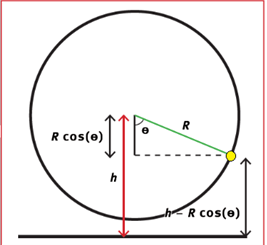
\includegraphics[width=.4\linewidth]{trigonometricas56}
\caption{Fonte: Soares (2010)}
\label{}
\end{figure}

\ifdefined\prof
\begin{solucao}

\begin{enumerate}
\item $h=h(\theta)=45{,}5-42{,}5\cos(\theta)$
\item $\theta(t)=t\frac{\pi}{0}$
\item $h(t)=45{,}5-42{,}5\cos(t\frac{\pi}{9})$
\end{enumerate}

\end{solucao}
\fi

\end{document}